%!TeX root = main.tex
%!encoding = UTF-8 Unicode

% \chapter{Methods for Measurement of EMC-Relevant Signal Components}
\chapter{Methodology for Measuring the EMC-Relevant Signal Components of Transient Switching Events}
\label{ch:Methods}

Accurate measurement of the EMC-relevant signal components of transient switching events is essential for characterizing the intrinsic EM emission behavior of power semiconductor devices.
Even when the conventional measurement errors discussed in Section~\ref{ch:MeasurementErrors} are minimized, these components can be obscured by thermal and quantization noise at high frequencies.
Dedicated measurement methods are therefore required to resolve the relevant signal components beyond the limitations of conventional measurement setups.

This chapter first reviews existing approaches to semiconductor-focused emission characterization and identifies the methodological gap addressed in this thesis.
It then quantifies the noise-induced limitations of conventional terminal measurements.
On this basis, it presents methods that combine analogue measurement techniques and digital signal processing to improve measurement accuracy at high frequencies.
Subsequently, methods for separating the spectral contributions of individual switching events are introduced to enable a more detailed analysis of EM noise generation.
The chapter concludes by defining figures of merit for evaluating the EMC-relevant characteristics of switching transients.


%!TeX root = main.tex
%!encoding = UTF-8 Unicode
\section{State of the Art and Research Gap in Semiconductor-Focused Emission Characterization}

As established in Chapter~\ref{ch:Fundamentals}, semiconductor switching generates the voltage and current transients that excite EM emissions, while the surrounding circuit determines their propagation to system-level measurement ports.
This distinction is also reflected in the literature on semiconductor-focused EMC analysis~\cite{hillenbrand_frequency_2016,takahashi_noise-source_2021,marlier_modeling_2012}.
Characterizing a device therefore requires distinguishing its switching-source spectra from the effects of the propagation path.
Here, intrinsic emission behavior denotes the terminal-level switching behavior under defined operating and circuit conditions, rather than a device property independent of its environment.

The present review focuses on approaches that relate EM emissions to semiconductor switching behavior, particularly the high-frequency switching behavior not captured by idealized pulse models~\cite{kragl_impact_2024}.
Three approaches are considered: system-level measurements, simulation-based analysis, and direct measurements at the device terminals.
They are assessed in terms of their ability to distinguish individual source contributions, resolve switching events, and characterize small high-frequency signal components.

\subsubsection*{System-Level Measurements}
In experimental system-level setups, various semiconductor technologies are tested within a commutation cell, and their emissions are compared using a LISN~\cite{apelsmeier_model_2020, takahashi_noise-source_2021, zhang_two-port_2020, tlig_conducted_2025, lemmon_methodology_2018, huber_ultra-low_2017} or antenna~\cite{radchenko_transfer_2014,domurat-linde_analysis_2012}. 
This approach enables comparisons of the system-level emissions obtained with different semiconductor technologies and provides a direct link to conventional EMC assessment.

However, the measured spectrum contains the combined contributions of all active noise sources after propagation through the surrounding circuit.
It does not, by itself, identify the contribution of an individual switch or switching event, which makes a detailed analysis challenging.
Additionally, within a given frequency range, the combined emissions can be dominated by a single switching event whose contribution at the measurement port substantially exceeds those of the other events.
If a parameter variation reduces the emissions associated with a weaker event while leaving the dominant contribution unchanged, the resulting change in the total level may be too small to distinguish in the logarithmic emission spectrum.
A beneficial effect on that event may therefore remain undetected in a system-level measurement, despite a substantial reduction in its individual contribution.

Furthermore, the measured emissions depend on the passive components and layout through their transfer functions~\cite{xie_high_2019,phukan_characterization_2023}.
Strong attenuation for a given frequency range along the propagation path can mask parameter-induced changes in the source spectrum.
A weak dependence of the measured emissions on a device parameter may therefore be misinterpreted as low sensitivity of the source itself to that parameter.
To account for the propagation-path influence, studies have reconstructed noise-source spectra from system-level measurements by deconvolving the propagation-path response.
While this approach provides satisfactory results at low frequencies, its accuracy in the higher-frequency range governed by the detailed switching transients remains insufficiently established.

\subsubsection*{Simulation-Based Approaches}
The limitations of system-level measurements make it difficult to determine which aspects of semiconductor switching behavior are responsible for a change in the measured emissions.
Simulation-based approaches provide both direct access to true device voltages and currents, and can model the propagation path to also predict the resulting system-level emissions, enabling a more comprehensive understanding of the relationship between device behavior and observed emissions.
In these studies, behavioral models are parameterized to identify which device properties drive emissions in specific frequency bands~\cite{hillenbrand_sensitivity_2017, kragl_semiconductor-focused_2025, liu_modeling_2016, yuan_emi_2015}.
Simulation permits individual device parameters and source contributions to be investigated separately, subject to the validity of the model and its representation of circuit parasitics.

However, these models are calibrated using conventional double-pulse tests and static measurements~\cite{van_der_broeck_simulating_2023,kragl_semiconductor-focused_2025}.
The resulting calibration data do not capture the small high-frequency signal components relevant to EMC when these fall below the measurement noise floor, as explained in Section~\ref{sec:MeasurementLimitation}.
Without this information, the models cannot be assumed to predict these components accurately.
Their behavior in this frequency range remains uncalibrated and unverified.
Accurate high-frequency voltage and current measurements are therefore needed to characterize the devices and validate the models.

\subsubsection*{Direct Measurements at Device Terminals}

Direct measurements at the device terminals provide the voltage and current signals needed for device characterization and model validation.
They allow the source spectra to be investigated without reconstructing them from system-level emissions or relying on a semiconductor model.

The main difficulty is resolving small high-frequency components within a large switching transient.
Conventional voltage measurements can become noise-limited above the device resonance frequency despite sufficient probe bandwidth~\cite{labrousse_switching_2011,kragl_impact_2024}.
Sufficient signal-to-noise ratio (SNR), rather than nominal bandwidth alone, is therefore essential.

To address this limitation,~\cite{oswald_high-bandwidth_2011} combined a passive voltage probe with a high-pass filter to measure high-frequency switching components in a discrete IGBT\@.
However, the approach was demonstrated only for IGBTs and for frequencies up to \SI{30}{MHz}.
The passive probe measured only the low-side drain-source voltage, providing access to just one of the three source signals in a switching cell: the high-side voltage, low-side voltage, and commutation current.

\subsubsection*{Research Gap and Methodological Requirements}
The remaining gap is a validated method for measuring all three source signals of a switching cell with sufficient SNR up to \SI{400}{MHz}.
These signals are the high-side voltage, low-side voltage, and commutation current.
The method must also separate the spectral contributions of individual switching events.
Measurements under defined operating and circuit conditions can then support device comparisons and model validation.

This thesis addresses this gap through measurement methods, sensors, and signal processing.
Section~\ref{sec:MeasurementLimitation} first explains the noise limits of conventional measurements.
The rest of this chapter develops methods to reduce the effects of measurement noise and separate switching events.
Chapter~\ref{ch:Sensors} presents the sensors, and Chapter~\ref{ch:Validation} validates the complete measurement setup.




%!TeX root = main.tex
%!encoding = UTF-8 Unicode
\section{Noise-Induced Measurement Limitations}
\label{sec:MeasurementLimitation}

To motivate the dedicated measurement approach, this section analyzes the noise-induced limitations that arise when a switching voltage waveform is measured with a conventional probe and digitized by an oscilloscope ADC\@.
These limitations are particularly significant for small, high-frequency signal components relevant to EMC analysis.
For conventional switching metrics, such as overvoltage, $\sddt{v}_\text{max}$, and switching energy, their influence is typically negligible under the measurement conditions considered.

\fref{fig:QuantNoise} illustrates these limitations in the time and frequency domains by comparing a simulated voltage transient with its quantized counterpart contaminated by thermal noise.
The spectral plot focuses on \SIrange{10}{500}{MHz}, where switching transients are particularly relevant to the electromagnetic emission behavior of power semiconductor devices.
Electromagnetic emissions from inverters remain relevant above this range; however, practical experience from measurements in the EMC chamber indicates that emissions above approximately \SI{500}{MHz} are often dominated by digital clocking in microcontrollers or FPGAs rather than by power semiconductor switching.
This frequency therefore serves as an empirical guideline for the scope of the present analysis, not as a strict boundary between emission sources.


\subsection{Thermal Noise}

Thermal noise arises from the random thermal motion of charge carriers in every resistive element of the measurement system.
The RMS thermal noise voltage across a resistance can be expressed as
\begin{equation}
	\mi{v}{n,th,RMS} = \sqrt{4 k_B T R \Delta f},
\end{equation}
where $k_B$ is the Boltzmann constant, $T$ is the absolute temperature, $R$ is the resistance, and $\Delta f$ is the measurement bandwidth.
Its power spectral density is approximately constant over the frequency range considered, so its RMS amplitude increases with the square root of the measurement bandwidth.

For the following analysis, the differential probe and oscilloscope are taken as the dominant sources of measurement noise.
Thermal noise from the device under test is neglected by approximating its drain-source impedance as an ideal capacitance with zero equivalent series resistance.

In the oscilloscope, resistive elements in the input attenuator and amplifier stages generate thermal noise, while the active circuitry introduces additional electronic noise.
The measured RMS noise depends on the selected vertical range, which determines the input attenuation and amplification.

In the differential probe, the resistive voltage divider and amplifier circuitry likewise contribute noise.
A higher probe attenuation reduces the signal reaching the oscilloscope, making the oscilloscope noise more significant when referred back to the measured voltage.

For both instruments, the analogue bandwidth determines the integrated noise level.
Reducing this bandwidth lowers the RMS noise, but also suppresses high-frequency signal components.
Since the present analysis requires accurate measurement of signal components up to \SI{500}{MHz}, bandwidth reduction cannot be used to lower the noise floor at the expense of the required frequency response.
The noise specifications must therefore be evaluated for the selected vertical range and probe attenuation, with sufficient analogue bandwidth to preserve these components.

The following calculation uses the noise values specified in the instrument datasheets: \SI{1.61}{mV} for the oscilloscope at \SI{100}{mV/div} and \SI{500}{MHz} bandwidth~\cite{tektronix_mso_2026} and \SI{55}{mV} for the differential probe at an attenuation ratio of \mti{a}{probe}~=~250~\cite{pmk_gmbh_datasheet_2017}.
These specifications include electronic noise contributions beyond purely thermal noise and are used here to estimate the analogue measurement noise floor.
For this estimate, both values are interpreted as RMS voltages, with the probe noise referred to its output and the oscilloscope noise referred to its input.
Assuming uncorrelated noise sources and a frequency-independent probe attenuation over the range considered, their noise powers add.
The combined RMS noise referred to the high-voltage side is therefore

\begin{equation}
	\mi{V}{n,th,RMS} = \mti{a}{probe}\sqrt{\mi{v}{n,th,osci}^2 + \mi{v}{n,th,probe}^2}
	\approx \SI{13.76}{V}.
\end{equation}

The symbol \mi{V}{n,th,RMS} denotes the combined analogue noise estimate, including the additional electronic noise contained in the datasheet specifications.
To estimate its contribution to the spectral noise floor, each source is approximated as white noise over its equivalent noise bandwidth.
The RMS noise in an FFT bin, referred to the high-voltage side, is then

\begin{equation}
	\mi{V}{th,bin,RMS} = \mti{a}{probe}\sqrt{
	\left(\frac{\mi{v}{n,th,osci}^2}{\mi{B}{n,osci}}
	+ \frac{\mi{v}{n,th,probe}^2}{\mi{B}{n,probe}}\right)\mi{B}{bin}},
	\label{eq:RMStoAmplitudePlot}
\end{equation}

Here, \mi{B}{n,osci} and \mi{B}{n,probe} are the equivalent noise bandwidths associated with the respective RMS specifications, including any subsequent filtering in the measurement chain.
If filtering changes a source's bandwidth, its integrated RMS noise must also be adjusted consistently.
These bandwidths depend on the analogue frequency responses and are not generally equal to the Nyquist frequency.
The nominal \SI{500}{MHz} oscilloscope bandwidth is a signal-bandwidth specification and need not equal its equivalent noise bandwidth.

The quantity \mi{B}{bin} is the equivalent noise bandwidth of the FFT window: for a rectangular window, it equals the bin spacing $\Delta \mi{f}{bin} = \mi{f}{s}/\mi{N}{FFT}$, while other windows require a window-dependent correction.
The estimate represents RMS noise per bin; comparison with the plotted FFT requires consistent window and amplitude normalization.
In logarithmic form, the RMS bin noise becomes
\begin{equation}
	\mi{V}{th,bin,RMS}^{\mathrm{dB}\upmu\mathrm{V}} = 20 \cdot \log_{10}\left(\frac{\mi{V}{th,bin,RMS}}{\SI{1}{\micro V}}\right).
\end{equation}

This analogue noise floor can mask small high-frequency signal components even when the measurement system provides sufficient signal bandwidth.









\subsection{Quantization Noise}
\label{sec:QuantNoise}

In addition to analogue noise, digitization by the oscilloscope introduces quantization error.
The oscilloscope's ADC represents each sampled input voltage by one of a finite number of discrete amplitude levels.
The difference between the input voltage and the assigned level is the quantization error; for ideal rounding without clipping, its magnitude is bounded by half the quantization step.
For a given ADC resolution, a wider input voltage range increases the spacing between these levels.
The vertical range required to capture the full switching transient therefore affects the resolution available for its small high-frequency components.

Quantization error is inherently signal-dependent and may produce discrete spectral components when its pattern repeats. 
For the following noise-floor estimate, however, it is approximated as uniformly distributed between adjacent quantization levels and uncorrelated with both the input signal and errors at other sampling instants. 
Under these assumptions, it can be modeled as additive white quantization noise.

The quantization process can be written as a rounding function that maps the input signal to the nearest quantization level:
\begin{equation}
	Q(\mi{v}{DS}) = \text{round}\left(\frac{\mi{v}{DS}}{q}\right) \cdot q,
	\label{eq:quantization}
\end{equation}

Here, $q$ is the ADC quantization step, calculated as
\begin{equation}
	q = \dfrac{\mi{V}{max}-\mi{V}{min}}{2^{\mti{N}{ENOB}}}.
\end{equation}

The effective number of bits (ENOB) is typically lower than the nominal ADC resolution (\mi{N}{ADC}) because of non-idealities in the sampling process, such as jitter, thermal noise, and other error sources. It also decreases with frequency~\cite{tektronix_mso_2026}.

Assuming a uniform distribution of the quantization error, the quantization noise is calculated as
\begin{equation}
	\mi{V}{quant,RMS} = \sqrt{\frac{q^2}{12}}
\end{equation}
The derivation of this expression is omitted here and can be found in~\cite{silicon_laboratories_an118_2013}.

For an ideal ADC with white, uncorrelated quantization error, the quantization noise is distributed over the Nyquist bandwidth $\mi{f}{s}/2$.
Using the same RMS-per-bin normalization as in Eq.~\ref{eq:RMStoAmplitudePlot}, its spectral contribution is
\begin{equation}
	\mi{V}{quant,bin,RMS} = \mi{V}{quant,RMS}\sqrt{\frac{\mi{B}{bin}}{\mi{f}{s}/2}},
\end{equation}
where the noise and signal amplitudes must be referred to the same point in the measurement chain.









\subsection{Implications for  Measurements of Switching Transient}

The analogue and quantization noise contributions jointly limit the spectral information that can be extracted from a measured switching transient.
Under the assumption of uncorrelated analogue and quantization noise, their RMS contributions within the same FFT bin combine as
\begin{equation}
	\mi{V}{noise,bin,RMS} = \sqrt{\mi{V}{quant,bin,RMS}^2 + \mi{V}{th,bin,RMS}^2},
\end{equation}
with both contributions referred to the same point in the measurement chain.
The following simulation illustrates the resulting limitations for a conventional probe and oscilloscope measurement chain.

\begin{figure}[!htbp]
	\begin{subfigure}{\textwidth}
		\centering
		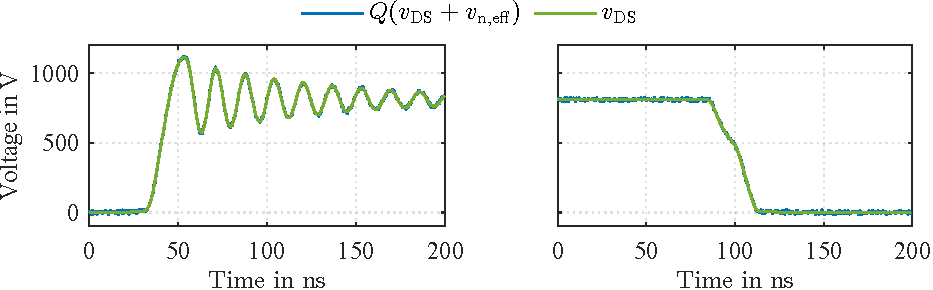
\includegraphics[scale = 1]{figures/3_Methods/Measurement_Limitation/DPT_TD_new.pdf}
		\caption{Simulated drain-source voltage switching transient in the time domain, with and without thermal and quantization noise (PSpice).}
	\end{subfigure}\par
	\vspace{1cm}\par
	\begin{subfigure}{\textwidth}
		\hspace{-0.7cm}
		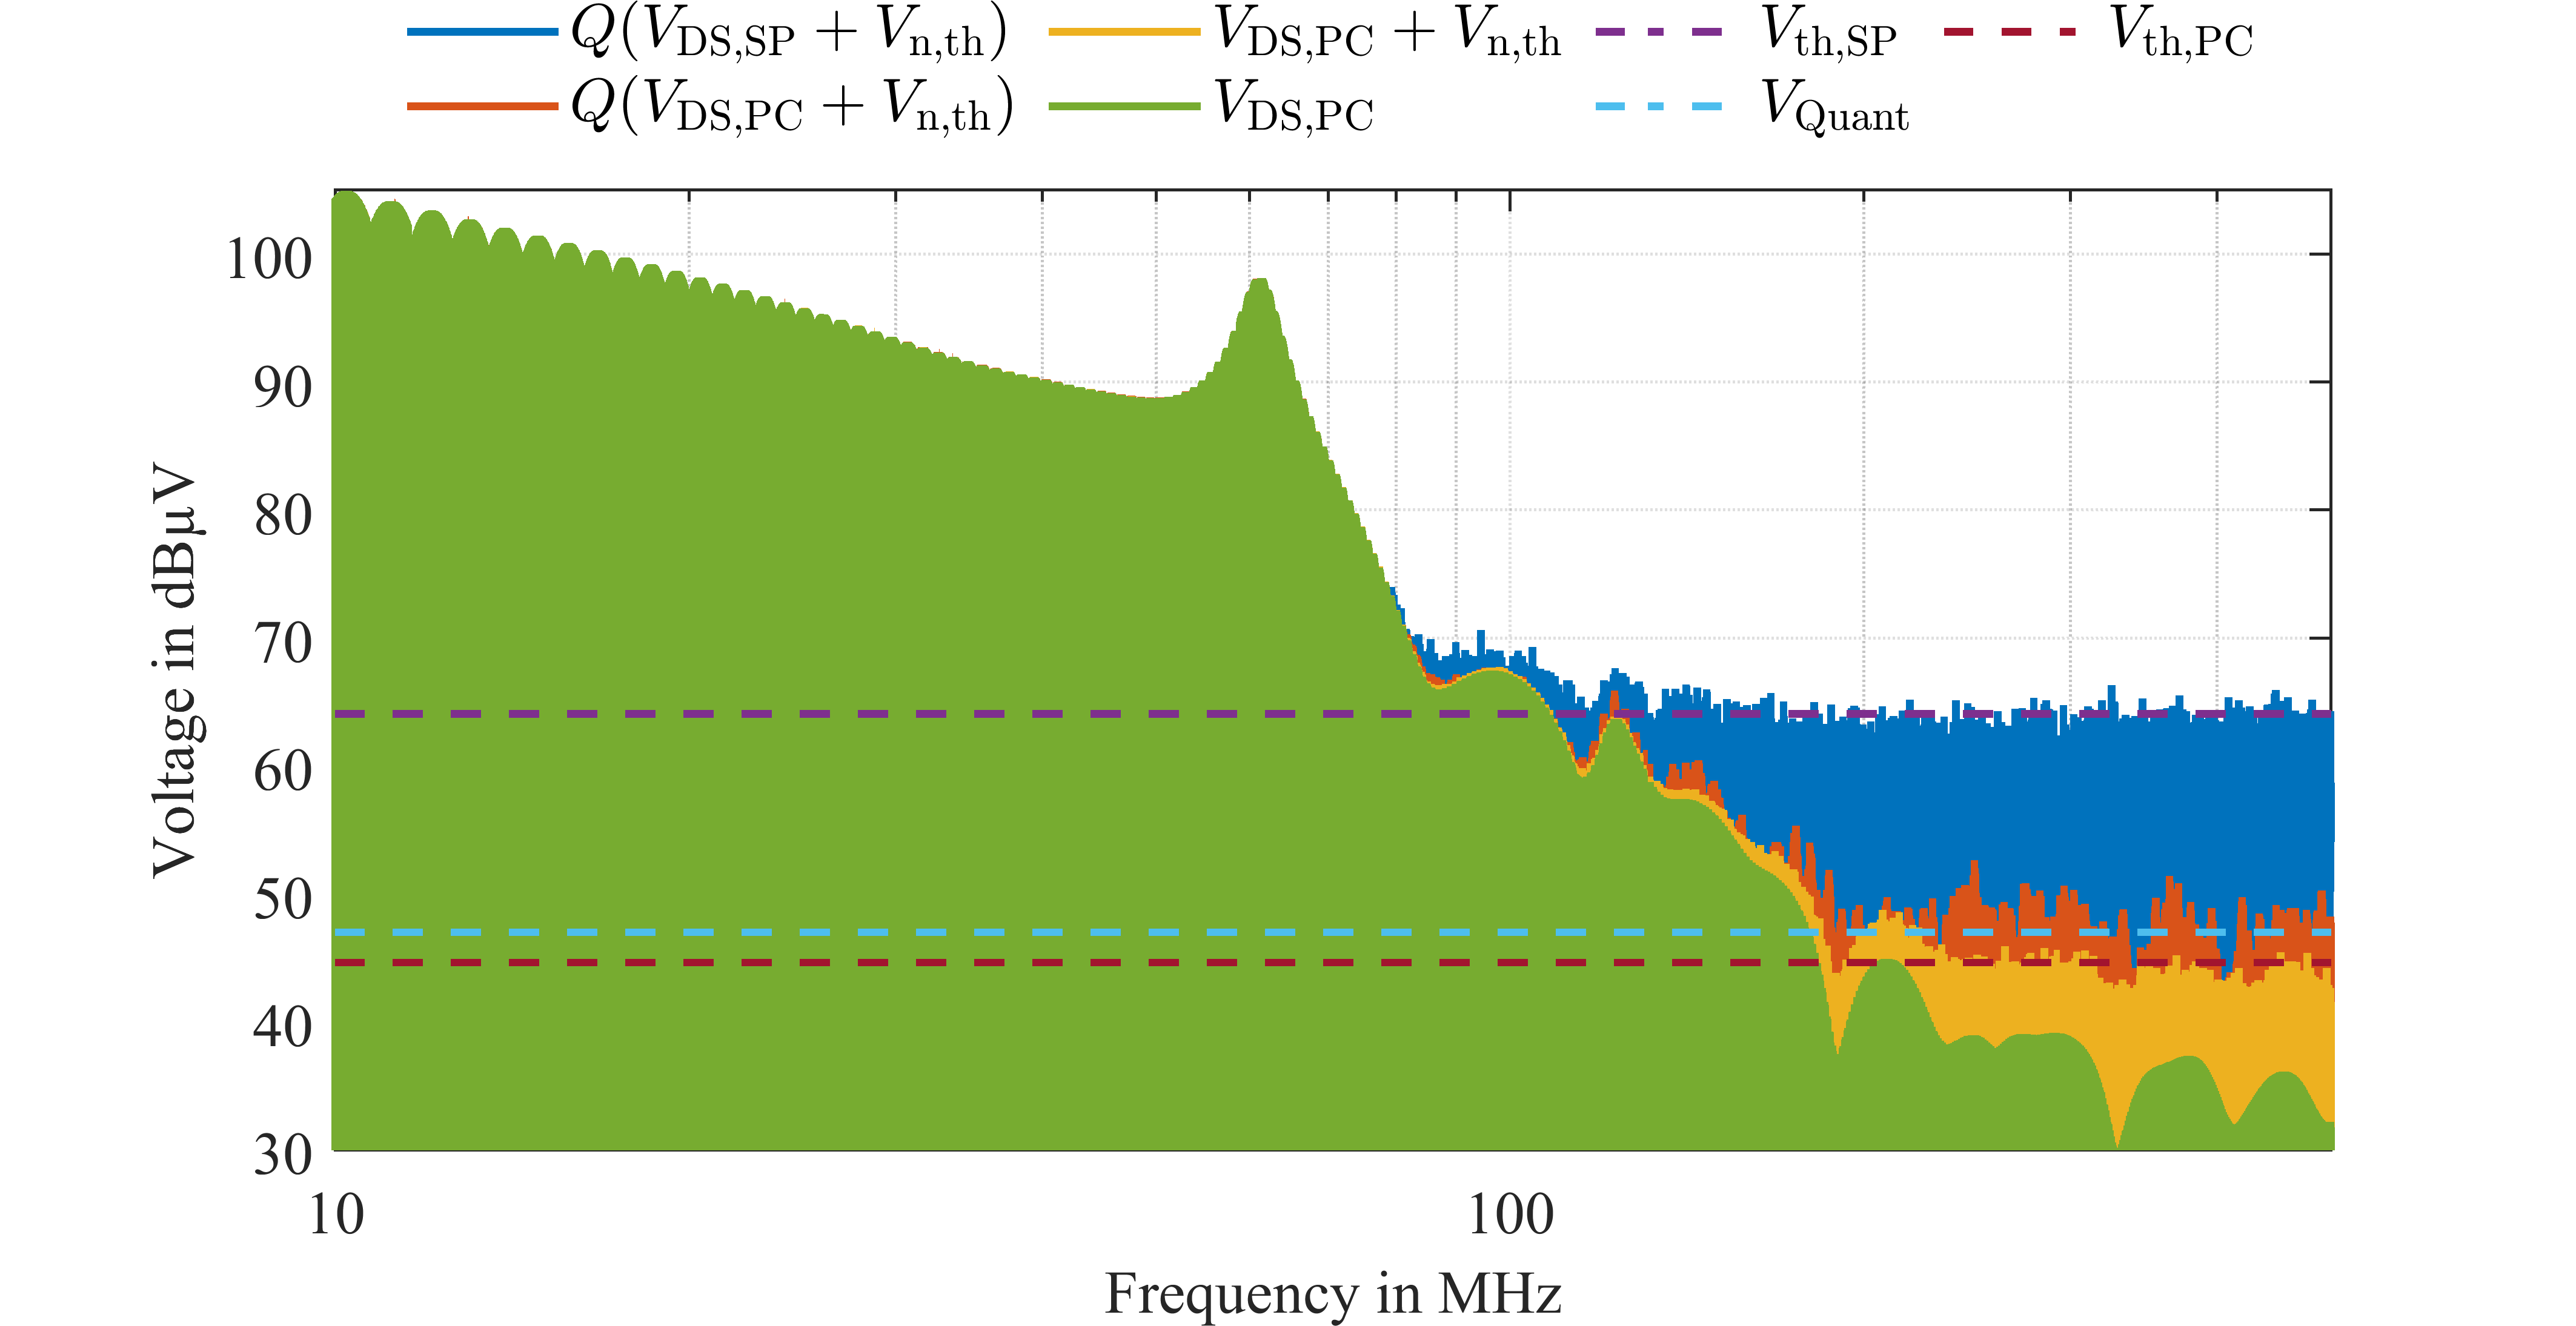
\includegraphics[scale = 1]{figures/3_Methods/Measurement_Limitation/DPT_FD_new.png}
		\caption{FFT of the simulated signal with and without thermal and quantization noise, shown for a single pulse (SP) and a pulse chain (PC). Calculated noise floors are added in dashed lines.}
	\end{subfigure}
	\caption{Noise-induced measurement limitations for switching transients in the time and frequency domains.}\label{fig:QuantNoise}
\end{figure}

Figure~\ref{fig:QuantNoise} compares the spectrum of the quantized, noise-contaminated single-pulse (SP) signal, $Q(\mi{V}{DS,SP}+\mi{V}{n,th})$, shown in blue, with that of the noise-free pulse-chain (PC) signal, $\mi{V}{DS,PC}$, shown in green.
The single-pulse signal represents a double-pulse test, which is commonly used to characterize power semiconductor devices.
The remaining spectra illustrate the effects of the measurement methods introduced in the following subsections to mitigate these noise limitations.

In the simulated single-pulse measurement, the signal spectrum falls below the noise floor at approximately \SI{80}{MHz}, above the resonance at \SI{62}{MHz}.
Beyond this frequency, the high-frequency voltage components cannot be reliably distinguished from measurement noise under the conditions considered.

The resonance is governed by the MOSFET output capacitance and commutation-loop inductance.
Typical resonance frequencies are approximately \SIrange{10}{50}{MHz} for modules and \SIrange{80}{120}{MHz} for discrete devices.

As discussed in Chapter~\ref{ch:Fundamentals}, finite switching transition times cause the high-frequency spectral envelope to decay, reducing the signal amplitudes available for measurement.
The noise-floor crossing therefore depends on both the signal spectrum and the measurement conditions; it is not fixed by the resonance frequency alone.

A numerical example illustrates the scale of these spectral amplitudes relative to an ENOB-based equivalent voltage step.
For unequal rise and fall times, the high-frequency spectral envelope can be estimated as~\cite{bi_prediction_2019}
\begin{equation}
	\mi{V}{DS,env}(f) = \dfrac{\mi{V}{DC}\mi{f}{sw}}{\uppi^2 f^2}
	\left(\dfrac{1}{\mi{\tau}{r}}+\dfrac{1}{\mi{\tau}{f}}\right),
	\quad f > \dfrac{1}{\uppi\min(\mi{\tau}{r},\mi{\tau}{f})}.
\end{equation}
With $\mi{V}{DC} = \SI{800}{V}$, $\mi{f}{sw} = \SI{25}{kHz}$, $\mi{\tau}{r} = \SI{20}{ns}$, and $\mi{\tau}{f} = \SI{50}{ns}$, the envelope at \SI{100}{MHz} is approximately \SI{14.2}{mV}.
For a probe attenuation of $\mti{a}{probe} = 250$, the corresponding envelope amplitude referred to the ADC input is
\begin{equation}
	\mi{v}{ADC,in} = \dfrac{\mi{V}{DS,env}(\SI{100}{MHz})}{\mti{a}{probe}}
	= \dfrac{\SI{14.2}{mV}}{250} \approx \SI{57}{\micro V}.
\end{equation}
For comparison, an assumed effective resolution of $\mti{N}{ENOB} = 14$ bits and an input range corresponding to \SI{-150}{V} to \SI{1200}{V} on the measured side yield an equivalent voltage step referred to the ADC input of
\begin{equation}
	\mi{q}{ADC,eff} = \dfrac{\mi{V}{max}-\mi{V}{min}}{\mti{a}{probe}\,2^{\mti{N}{ENOB}}}
	= \dfrac{\SI{1200}{V}-(\SI{-150}{V})}{250\cdot 2^{14}}
	\approx \SI{330}{\micro V}.
\end{equation}
The estimated signal amplitude is approximately six times smaller than the equivalent voltage step, placing both within one order of magnitude and illustrating the resolution challenge.

These small high-frequency voltage components are primarily relevant to EMC analysis.
Under the measurement conditions considered, their influence on conventional metrics such as overvoltage, switching energy, and $\sddt{v}_\text{max}$ is typically negligible.
Characterizing SiC MOSFETs over the EMC-relevant frequency range of \SIrange{10}{500}{MHz} therefore requires methods that reduce these noise limitations while preserving the required signal bandwidth.
The following subsections introduce the corresponding measurement methods.
%!TeX root = main.tex
%!encoding = UTF-8 Unicode
\section{Analog Methods for EMC-Relevant Signal Measurement}

Resolving small EMC-relevant signal components at high frequencies requires measurement methods that address both thermal and quantization noise.
This section first examines the potential and limitations of oversampling and averaging for reducing the thermal-noise floor.
It then introduces an analog high-pass measurement method to mitigate quantization-noise limitations.
By attenuating the dominant low-frequency components before digitization, this method enables more effective use of the available ADC range for the high-frequency components of interest.

\subsection{Oversampling and Pulse-Chain Acquisition}
Section~\ref{sec:MeasurementLimitation} showed that the noise floor of a conventional measurement chain can obscure small high-frequency components of the switching voltage.
Before introducing a dedicated analog measurement method, the extent to which conventional noise reduction are considered.
Two approaches are distinguished: oversampling with subsequent bandwidth-limited averaging, and spectral evaluation of a longer record containing repeated switching pulses.

\subsubsection*{Oversampling:}
Oversampling acquires the signal at a sampling frequency higher than the minimum required by the analysis bandwidth.
Subsequent low-pass filtering and averaging suppress noise outside this bandwidth while retaining the signal components of interest.
For an ideal ADC with white, uncorrelated quantization error, the corresponding effective number of bits (ENOB) is~\cite{silicon_laboratories_an118_2013}

\begin{equation}
	\mti{N}{ENOB} = \mti{N}{ADC} + 0.5\cdot \log_2\left(\frac{\mi{f}{s}}{2\mi{f}{max}}\right).
\end{equation}

Here, \mti{N}{ADC} is the nominal ADC resolution, \mi{f}{s} is the sampling frequency, and \mi{f}{max} is the highest frequency of interest.
With \eref{eq:quantization}, this can be translated into an effective quantization step.

The argument of the logarithm $(\sfrac{\mi{f}{s}}{2\mi{f}{max}})$ is the oversampling factor, with the factor of two following from the Nyquist criterion.
For the present analysis, the required bandwidth is set to $\mi{f}{max} = \SI{500}{MHz}$, whereas \mi{f}{s} is limited by the maximum sampling rate of the oscilloscope.

The oscilloscope achieves its high sampling rate by using time-interleaved ADCs.
These converters sample the same input signal at staggered sampling instants, and their outputs are combined into a single sample sequence with a higher aggregate sampling rate.
Modern oscilloscopes will typically preset the high resolution mode to provide optimal oversampling and averaging settings automatically.

\subsubsection*{Pulse-Chain Acquisition:}
Whereas oversampling uses a higher sampling frequency relative to the required signal bandwidth, a complementary approach reduces the spectral noise floor by extending the acquisition duration.
For a repeatable switching waveform, this is achieved by recording a pulse chain (PC) containing $M$ repetitions instead of a single pulse (SP).
At an unchanged sampling frequency, the acquisition duration and record length therefore increase by a factor of $M$.
For the same FFT window type, the equivalent noise bandwidth of each bin decreases by this factor.
According to Eq.~\ref{eq:RMStoAmplitudePlot}, the RMS thermal-noise contribution per bin consequently becomes

\begin{equation}
	\mi{V}{th,PC} = \frac{\mi{V}{th,SP}}{\sqrt{M}}.
\end{equation}

This reduction concerns the spectral noise per bin, not the total time-domain RMS noise.
For repeatable switching pulses and coherent acquisition with consistent amplitude normalization, the spectral components at multiples of \mi{f}{sw} retain their amplitudes, whereas the uncorrelated noise contribution per bin decreases.
The thermal-noise-limited SNR therefore improves by a factor of $\sqrt{M}$.
In practice, the usable record length is constrained by the oscilloscope acquisition memory and by the requirement that the switching conditions remain unchanged throughout the pulse chain.

The pulse-chain spectra in Fig.~\ref{fig:QuantNoise}, illustrate this improvement for $M=100$.
The quantized single-pulse spectrum, $Q(\mi{V}{DS,SP}+\mi{V}{n,th})$, is shown in blue, while the quantized pulse-chain spectrum, $Q(\mi{V}{DS,PC}+\mi{V}{n,th})$, is shown in orange.
Their comparison shows an SNR improvement of approximately \SI{20}{dB} in the thermal-noise-dominated region, consistent with the expected factor of $\sqrt{100}=10$.
The corresponding non-quantized pulse-chain spectrum, $\mi{V}{DS,PC}+\mi{V}{n,th}$, shown in yellow, still exhibits a lower noise floor than its quantized counterpart, demonstrating the remaining contribution of quantization noise.

However, once thermal noise is sufficiently suppressed in the simulation considered here, quantization noise becomes dominant and limits further improvement.
The introduced noise reduction alone therefore do not ensure that the small signal components can be resolved over the full EMC-relevant frequency range.
The following subsection introduces high-pass measurement to make more effective use of the ADC input range for these components before digitization.

%!TeX root = main.tex
%!encoding = UTF-8 Unicode

\subsection{High-Pass Measurement}
To mitigate the remaining quantization-noise limitations, a high-pass filter is applied before digitization.
By attenuating the dominant low-frequency components, the filter allows a smaller ADC input range to be selected.
The principle is to counteract the \SI{-40}{dB/dec} decay of the high-frequency switching spectrum (see \fref{fig:Diss_SpectrumCreation_firstOrder}) using a high-pass transfer function with a \SI{+40}{dB/dec} slope.
The resulting spectral envelope at the ADC input is approximately flat over this frequency range, enabling more uniform use of the available ADC dynamic range and improving the SNR of the high-frequency components relative to the quantization-noise floor.
The filtered spectrum is then compensated in post-processing to recover the original voltage spectrum within the usable measurement bandwidth, as illustrated in Fig.~\ref{fig:QuantNoise_wHP}.

\begin{figure}[!htb]
	\centering
	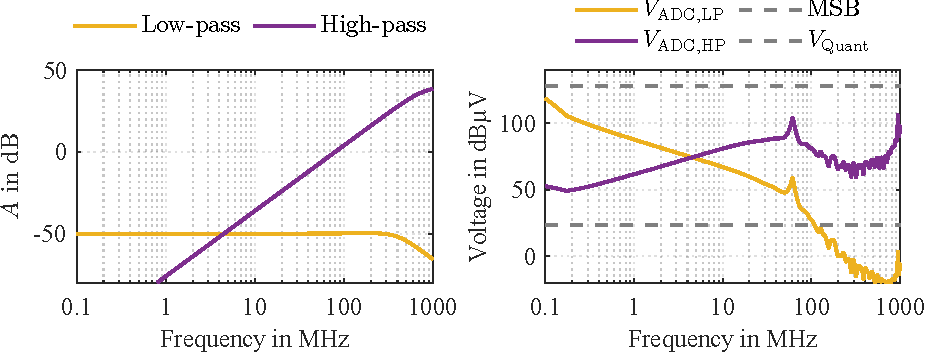
\includegraphics[scale = 1]{figures/3_Methods/Highpass/Method_Highpass_comb.pdf}
	\caption{High-pass measurement principle for EMC-relevant components of a switching transient. Left: Transfer functions of a conventional low-pass measurement and a second-order high-pass measurement. Right: Corresponding voltage spectra at the oscilloscope input and their respective quantization-noise floors.}\label{fig:QuantNoise_wHP}
\end{figure}

For this compensation, the high-pass probe is modeled as a linear time-invariant (LTI) system with impulse response $\mi{a}{HP}(t)$ and frequency-domain transfer function $\mi{A}{HP}(f)$.
At the oscilloscope input, the measured signal is the convolution of the drain-source voltage with the probe response:
\begin{equation}
	\mi{v}{DS,HP,raw}(t) = \mi{a}{HP}(t) \ast \mi{v}{DS}(t),
\end{equation}

which in the frequency domain becomes a multiplication:
\begin{equation}
	\mi{V}{DS,HP,raw}(f) = \mi{A}{HP}(f) \cdot \mi{V}{DS}(f).
\end{equation}

To recover the original drain-source voltage spectrum within the usable bandwidth, the measured spectrum is divided by the transfer function:
\begin{equation}
	\mi{V}{DS,HP,comp}(f) = \frac{\mathcal{F}\{\mi{v}{DS,HP,raw}(t)\}}{\mi{A}{HP}(f)} = \frac{\mi{V}{DS,HP,raw}(f)}{\mi{A}{HP}(f)}.
	\label{eq:HP_comp}
\end{equation}

For the spectral magnitude in logarithmic representation, this division corresponds to a subtraction of the probe gain $\mi{A}{HP}(f)$:
\begin{equation}
	\mi{V}{DS,HP,comp}^{\text{dB}\upmu\text{V}} = \mi{V}{DS,HP,raw}^{\text{dB}\upmu\text{V}} - \mi{A}{HP}^{\text{dB}}.
\end{equation}

High-pass measurement can therefore extend the usable frequency range beyond the noise-floor crossing of the conventional measurement.
Within the probe bandwidth, the achievable improvement remains limited primarily by the noise of the measurement chain, including any additional noise introduced by the high-pass circuitry.
%!TeX root = main.tex
%!encoding = UTF-8 Unicode

\section{Digital Processing for EMC-Relevant Signal Analysis}

Following acquisition, digital processing serves two complementary purposes: reducing the noise contribution in the measured waveform and enabling a more detailed analysis of the intrinsic EM emission behavior of power semiconductor devices.
This section first introduces a time-dependent noise filter for noise reduction and then presents an event-resolved spectral separation method that distinguishes the EMC-relevant contributions of individual switching events.

\subsection{Time-Dependent Noise Filter}

Up to this point, the noise-mitigation steps are generally applicable to arbitrary signals.
Further noise reduction is possible because the EMC-relevant voltage components are concentrated within a limited time interval around the switching event.
Based on this observation, a time-dependent noise filter is introduced that suppresses noise outside the transient, as illustrated for the low-pass signal in Fig.~\ref{fig:TDF}.
In the measurement procedure, the low-pass waveform is used to locate the switching transients, while the filter is applied to the high-pass waveform before spectral evaluation.

\begin{figure}[ht]
	\centering
	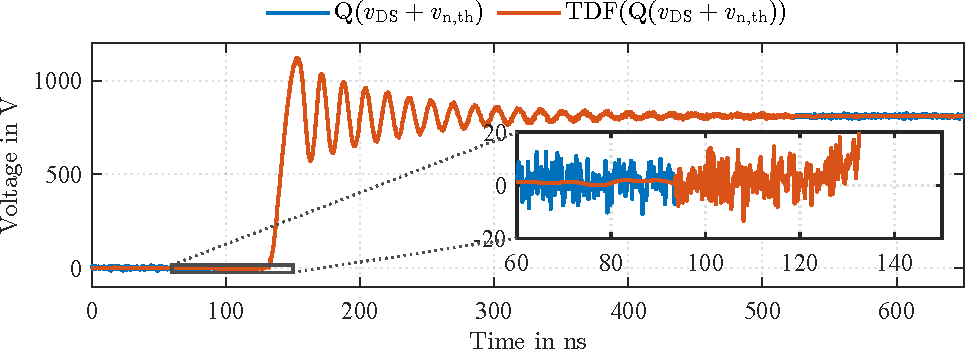
\includegraphics[scale = 1]{figures/3_Methods/TDF/DPT_TD_TDF2.pdf}
	\caption{Time-dependent noise filter to reduce noise outside the switching transient.}\label{fig:TDF}
\end{figure}

First, the transient midpoint \mi{t}{tr} is defined as the time instant at which the drain-source voltage reaches 50\% of its transition between the pre- and post-switching levels.
An asymmetric time interval \mi{I}{TDF} is then defined around \mi{t}{tr}.
It extends from \mi{T}{TDF}/5 before \mi{t}{tr} to 4\mi{T}{TDF}/5 after \mi{t}{tr}:

\begin{equation}
	\mi{I}{TDF} = \left[\mi{t}{tr}-\frac{\mi{T}{TDF}}{5},\,\mi{t}{tr}+\frac{4\mi{T}{TDF}}{5}\right].
\end{equation}

In this work, the window length \mi{T}{TDF} is set to \SI{500}{ns}, but it should be adjusted to approximately match the observed settling time of the resonant oscillation for the specific device under test.

Strong low-pass filtering is applied outside this interval, while the signal within it remains unfiltered.
For an input waveform $s(t)$, the filtered waveform is defined as

\begin{equation}
	\text{TDF}(s) =
	\begin{cases}
		s(t), & t \in \mi{I}{TDF} \\
		\mi{h}{LP,TDF}(t)\ast s(t), & t \notin \mi{I}{TDF}
	\end{cases}.
\end{equation}

Here, $\mi{h}{LP,TDF}(t)$ is the impulse response of a second-order Butterworth low-pass filter with a cutoff frequency of \SI{1}{MHz}.
The interval is defined separately for each switching transient.
At the interval boundaries, discontinuities between the filtered and unfiltered waveforms should be avoided to prevent additional spectral components.
Alternatively, stronger low-pass filtering or setting the signal to zero outside the transient intervals could be considered, provided that discontinuities at the interval boundaries are avoided.

For approximately white, uncorrelated noise, and neglecting the residual filtered noise outside the transient intervals, the RMS spectral noise per bin in the frequency range well above the filter cutoff can be approximated as

\begin{equation}
	\mi{V}{n,th,TDF} = \frac{\mi{T}{TDF}}{\mi{T}{sw}} \cdot \mi{V}{n,th}
\end{equation}

%!TeX root = main.tex
%!encoding = UTF-8 Unicode

\subsection{Event-Resolved Spectral Separation of Switching Transients}
\label{subsec:SpectralSeparation}
Whereas the time-dependent noise filter improves the SNR of the measured waveform, event-resolved spectral separation distinguishes the contributions of individual switching transients.

In power electronics analysis, it is standard practice to evaluate the four distinct switching transients separately: active-on (device turn-on), active-off (device turn-off), passive-on (body-diode turn-on), and passive-off (body-diode turn-off)~\cite{fritz_toward_2020}. 
Here, the active device initiates the transient while the passive device (conducting body diode) is turned off during commutation.

For EMC analysis, this separation is particularly valuable: it identifies which switching event dominates in each frequency band, enabling targeted understanding of noise generation mechanisms. 
Direct measurement at the semiconductor ports enables this separation, a key advantage of the methodology presented in this thesis unavailable in conventional system level EMC measurements, which capture only the aggregated noise from all events.

 \begin{figure*}[htb]
	\centering
	\begin{subfigure}{0.48\textwidth}
		\centering
		\input{"3_Methods/SnapNMirror/DPT_TD.tex"}
		\caption{Time domain simulation of double pulse test.}
	\end{subfigure} %
	\hfill
	\begin{subfigure}{0.48\textwidth}
		\centering
		\input{"3_Methods/SnapNMirror/DPT_FD.tex"}
		\caption{Frequency spectrum of simulated double pulse test.}
	\end{subfigure} %
	\begin{subfigure}{0.48\textwidth}
		\centering
		\input{"3_Methods/SnapNMirror/Snapped_TD.tex"}
		\caption{Four synthetic signals containing frequency components of one switching event only.}
	\end{subfigure}
	\hfill
	\begin{subfigure}{0.48\textwidth}
		\centering
		\raisebox{-2mm}[0pt][0pt]{\input{"3_Methods/SnapNMirror/Snapped_FD.tex"}}
		\caption{Frequency spectrum envelopes of all four switching events separated.}
	\end{subfigure}
	\caption{Methodology of the snap-and-mirror function for separated EMC analysis of all four switching events.}\label{fig:SnapNMirror}
\end{figure*}


To achieve event-resolved separation in the frequency domain, the snap-and-mirror method is applied~\cite{kragl_impact_2024}, whose operating principle is shown in \fref{fig:SnapNMirror}. 
The method identifies the midpoints of each switching cycle \mi{t}{m,n} and mirrors the measured signal around these points to produce four synthetic signals, one for each event type. This transformation is expressed as

\begin{equation}
	s_\mathrm{new}(t) = 
	\begin{cases}
		s(t) 					 		& \text{, for } \mi{t}{m,n}~~~< t < \mi{t}{m,n+1} \\
		s(-t + 2\cdot\mi{t}{m,n+1}) 	& \text{, for } \mi{t}{m,n+1} < t < \mi{t}{m,n+2} \\
		s(t) 					 		& \text{, for } \mi{t}{m,n+2} < t < \mi{t}{m,n+3} \\
		s(-t + 2\cdot\mi{t}{m,n+3}) 	& \text{, for } \mi{t}{m,n+3} < t < \mi{t}{m,n+4} \\
		\cdots
	\end{cases}
	\label{eq:snap}
\end{equation}

This transformation is valid for amplitude-spectrum analysis because time mirroring and shifting affect only the phase of the Fourier transform, not its magnitude. Specifically:

\begin{equation}
	\mathcal{F}\{s(-t)\} = S(-f) = S^\ast(f)
\end{equation}

\begin{equation}
	\mathcal{F}\{s(t-\mi{t}{0})\} = S(f)e^{-j\omega \mi{t}{0}}
\end{equation}

Therefore, the amplitude spectrum $|S(f)|$ remains unchanged. 

When the four event-resolved spectra are compared with the spectrum of the original voltage waveform, a peak detector is preferred. 
Each switching event occurs once per switching period in the original waveform but twice per switching period in the corresponding synthetic signal. 
Consequently, a conventional FFT or an averaged spectrum can give disproportionate weight to repeated transient contributions, increasing the apparent spectral magnitude by up to a factor of two. 
Peak detection retains the maximum level at each frequency rather than averaging these differently weighted contributions, making it better suited to this comparison.




%!TeX root = main.tex
%!encoding = UTF-8 Unicode

\section{Figures of Merit for Electromagnetic Emission Spectra}
A figure of merit (FOM) is a single quantitative value used to characterize the performance of a system, device, or process with respect to a defined objective. 
It condenses relevant performance into a value that can be compared across designs or operating conditions. 
In this thesis, FOMs are used to assess and compare the EMC-relevant performance of switching transients. 
They may be derived from the time-domain waveform, the frequency-domain spectrum, or both, and applied to comparisons across operating points, parameter variations, or changes over time. 
When such a sweep includes many conditions, direct comparison of all corresponding spectra can become challenging, and FOMs provide a compact basis for comparison. 
However, a single value cannot represent all information in a waveform or spectrum: each FOM comes at the cost of a loss of information.

The FOMs considered here cover time-domain, hybrid, and frequency-domain characteristics. 
The Heisenberg-Gabor Inequality combines temporal and spectral characteristics, while the frequency-domain FOMs describe broadband behavior or focus on selected frequencies, including resonances between the semiconductor output capacitance and the parasitic inductance of the commutation cell.

\subsubsection*{Rise time {\boldmath\mi{t}{10-90\%}}}
For transients with the same overall shape, rise time provides a useful basis for comparison because the second spectral corner shifts to lower frequencies as the transition duration increases, as described by \eref{eq:fc2_rise_time} and illustrated in \fref{fig:Diss_SpectrumCreation_firstOrder}. 
However, rise time alone does not characterize waveform shape and is therefore insufficient for reliable comparisons between different transient types, such as active-off and passive-off events, or between operating conditions when a parameter change alters the transient shape. 
Piecewise-linear and Gaussian-smoothed transitions can have substantially different spectral decay even at the same rise time; the contrast is illustrated in \fref{fig:Diss_SpectrumCreation_Heisenberg}, and reflected in \eref{eq:gaussian_spectrum}.



\subsubsection*{Maximum Slew Rate {$\boldmath\sddt{v}_\mathrm{max}$}}
The maximum voltage slew rate, $\sddt{v}_\mathrm{max}$, quantifies the steepest rate of voltage change during a switching transient. 
However, it does not map directly to a spectral behavior; its value is influenced by the voltage change, related to the DC-link voltage \mi{V}{DC}, and by the transition duration, related to the rise time \mi{t}{10-90\%}. 
Like the rise time, it is therefore most useful for comparing transients of similar shape.

Although slew rate is commonly used to quantify switching-related EM emissions, the author considers it unsuitable for this purpose. 
Instead, it should only be used when specifying driver-isolation requirements. 
A voltage transient across the isolation capacitance generates a displacement current, $i = C_\mathrm{iso}\sfrac{\mathrm{d}v}{\mathrm{d}t}$, which can interfere with the driver's normal operation.

\subsubsection*{Heisenberg-Gabor Inequality (HGI)}
As discussed in Section~\ref{sec:Fundamental_Generation}, a Gaussian-smoothed switching transient has been proposed as a theoretically EM-noise-optimal waveform. 
The Heisenberg-Gabor Inequality (HGI) uses this optimum as a reference for assessing switching transients based on their temporal and spectral dispersion~\cite{patin_power_2015,martinez-padron_definition_2022}. 
The Gaussian smoothing function is
\begin{equation}
	g(t) = \frac{1}{\sigma_t \sqrt{2\pi}}\cdot e^{-\dfrac{t^2}{2\sigma_t^2}},
\end{equation}
where the resulting semiconductor voltage follows from the convolution
\begin{equation}
	\mi{v}{DS,opt} = \mi{V}{DC}\cdot\mathrm{rect}(\frac{t}{\mathrm{d}T_\mathrm{s}}) * g(t)
\end{equation}
The resulting waveform for $\sigma_t = \SI{10}{ns}$ is shown in Fig. \ref{fig:IdealVsReal}.

The dispersions are calculated from the transient function $\lambda = \frac{\text{d}\mi{v}{DS}}{\text{d}t}$, the derivative of the voltage transient.

\begin{equation}
	\sigma_t = \sqrt{\frac{\int (t-\mi{t}{b})^2 \cdot |\lambda(t)|^2 \text{d}t}{\int |\lambda(t)|^2 \text{d}t}}\text{, with } \mi{t}{b} = \int t\cdot\lambda(t) \text{d}t
\end{equation}

\begin{equation}
\sigma_f = \sqrt{\frac{\int (\omega-\mi{\omega}{b})^2 \cdot |\Lambda(t)|^2 \text{d}\omega}{\int |\Lambda(t)|^2 \text{d}\omega}}\text{, with } \mi{\omega}{b} = \int \omega\cdot\Lambda(t) \text{d}\omega
\end{equation}

Here, $\Lambda(\omega)$ is the Fourier Transform of $\lambda(t)$.
Both can be used to calculate the FOM 
\begin{equation}
	HGI = \sigma_f \cdot \sigma_t \geq 0.5.
\end{equation}

The lower bound of 0.5 is attained by a Gaussian waveform. 
HGI therefore indicates the time--frequency spread product of the transient relative to this theoretical limit; a larger value corresponds to a larger product, not necessarily to greater high-frequency emission in every frequency band.

\subsubsection*{Band-Averaged Spectral Magnitude {\boldmath$\bar{V}_{\Delta f}$}}
To quantify broadband emission over a selected frequency band, the frequency-bin-width-weighted mean of the spectral magnitudes is defined as:

\begin{equation}
	\bar{v}_{10-150 \mathrm{MHz}} = \frac{1}{\Delta f_{tot}} \sum_{n = n_{10 \mathrm{MHz}}}^{n_{150 \mathrm{MHz}}} \Delta f_n \cdot a_n
\end{equation}

Here, $a_n$ is the magnitude of the Fourier coefficient in frequency bin $n$, $\Delta f_n$ is the width of that bin, and $\Delta f_{tot}=\sum_n\Delta f_n$ is the total bandwidth. 
The lower and upper frequency limits are selected for the region of interest, taking into account \mi{f}{sw} and \mi{f}{res}; the equation above uses the band from \SI{10}{MHz} to \SI{150}{MHz}.

\subsubsection*{Amplitude of Resonance Frequency {\boldmath$\hat{V}_\mathrm{res}$}}
Peaks in the emission spectrum may originate from the source spectrum of \mi{v}{DS} or from resonances in the transfer function introduced by passive components and layout parasitics. 
The resonance FOM, $\hat{V}_\mathrm{res}$, quantifies the spectral component at a selected resonance frequency.
Most of the time, this will be the main resonance, which is created by the oscillation between the output capacitance of the turned-off device and the parasitic inductance of the commutation loop.

\subsubsection*{Summary of FOMs}
The considered FOMs and the information they provide are summarized in Tab. \ref{tab:FOMs}; their influence on the spectrum is illustrated in Fig. \ref{fig:FOM_in_spectrum}.


\begin{table}[ht]
	\centering
	\caption{Summary of all considered FOMs for the emitted-noise performance of a switching event.}
	\begin{tabular}{c|c|c}		
		FOM	& domain &  information \\
		\hline
		\mi{t}{10-90\%} & time & $2^\mathrm{nd}$ cut-off frequency \\
		$\sddt{v}_\mathrm{max}$ & time & correlates with \mi{V}{DC} \& \mi{t}{10-90\%}\\
		HGI & hybrid & difference to EMC optimum \\
		$\bar{V}_{\Delta f}$ & frequency & total noise emission \\
		$\hat{V}_\mathrm{res}$ & frequency & resonance \\
	\end{tabular}
	\label{tab:FOMs}
\end{table}

\begin{figure}
	\centering\import{./figures/3_Methods/FOM/}{Diss_FOM_in_Spectrum.pdf_tex}
	\caption{Influence of FOM in spectrum.}
	\label{fig:FOM_in_spectrum}
\end{figure}
\FloatBarrier


\subsubsection*{Time-Resolved Frequency-Domain Analysis}
When a parameter varies during a measurement, the frequency-domain FOMs can be evaluated over time to track the corresponding changes in the emission spectrum. 
A spectrum calculated over the entire record would combine measurements from different parameter values and obscure this evolution. 
Because the spectrum also depends on the switching duty cycle, it is not meaningful to calculate these FOMs from an isolated transient. 
Instead, a moving window is used to calculate the spectrum over $n$ switching periods while separating consecutive events, as illustrated in \fref{fig:Moving_FD_FOM}, and the resulting signal segment is repeated to provide sufficient length for the FFT. 
This procedure can be applied either to the original waveform or to event-separated signals generated by the snap-and-mirror method.

\begin{figure}
	\centering\import{./figures/3_Methods/FOM/}{Moving_FD_FOM.pdf_tex}
	\caption{Moving window for calculation of FD FOM over time with a window length of n = 1.}
	\label{fig:Moving_FD_FOM}
\end{figure}











